% VLDB template version of 2020-08-03 enhances the ACM template, version 1.7.0:
% https://www.acm.org/publications/proceedings-template
% The ACM Latex guide provides further information about the ACM template

\documentclass[sigconf,nonacm]{acmart}

%% The following content must be adapted for the final version
% paper-specific
\newcommand\vldbdoi{XX.XX/XXX.XX}
\newcommand\vldbpages{XXX-XXX}
% issue-specific
\newcommand\vldbvolume{18}
\newcommand\vldbissue{1}
\newcommand\vldbyear{2025}
% should be fine as it is
\newcommand\vldbauthors{\authors}
\newcommand\vldbtitle{\shorttitle} 
% leave empty if no availability url should be set
\newcommand\vldbavailabilityurl{https://github.com/n3slami/Sketchbook.git}
% whether page numbers should be shown or not, use 'plain' for review versions, 'empty' for camera ready
\newcommand\vldbpagestyle{plain} 

\usepackage{array}
\usepackage{breqn}
\usepackage{booktabs,makecell}
\usepackage{enumitem}
\usepackage{tikz,pgfplots}
\usetikzlibrary{positioning}
\usetikzlibrary{arrows}
\usetikzlibrary{patterns}
\usetikzlibrary{shapes.geometric}
\usetikzlibrary{decorations.pathreplacing}
\usetikzlibrary{calligraphy}
\usetikzlibrary{hobby}
\usetikzlibrary{calc}

\usepackage{pifont}
\newcommand{\cmark}{\ding{51}}
\newcommand{\xmark}{\ding{55}}

\usepackage{thm-restate}
\newtheorem{theorem}{Theorem}[section]
\newtheorem{corollary}{Corollary}[theorem]
\newtheorem{lemma}[theorem]{Lemma}
\newtheorem{claim}[theorem]{Claim}

\usepackage{cleveref}

\graphicspath{{./figures/}}

\begin{document}
\title{Sketchbook: Expanding Sketches in Multiple Dimensions}

%%
%% The "author" command and its associated commands are used to define the authors and their affiliations.
\author{Navid Eslami}
\email{navideslami@cs.toronto.edu}
\affiliation{%
  \institution{University of Toronto}
  \city{Toronto}
  \country{Canada}
}

\author{Ioana O. Bercea}
\email{bercea@kth.se}
\affiliation{%
  \institution{KTH Royal Institute of Technology}
  \city{Stockholm}
  \country{Sweden}
}

\author{Rasmus Pagh}
\email{pagh@di.ku.dk}
\affiliation{%
  \institution{University of Copenhagen}
  \city{Copenhagen}
  \country{Denmark}
}

\author{Niv Dayan}
\email{nivdayan@cs.toronto.edu}
\affiliation{%
  \institution{University of Toronto}
  \city{Toronto}
  \country{Canada}
}

%%
%% The abstract is a short summary of the work to be presented in the
%% article.
\begin{abstract}
\end{abstract}

\maketitle

%%% do not modify the following VLDB block %%
%%% VLDB block start %%%
\pagestyle{\vldbpagestyle}
\begingroup\small\noindent\raggedright\textbf{PVLDB Reference Format:}\\
\vldbauthors. \vldbtitle. PVLDB, \vldbvolume(\vldbissue): \vldbpages, \vldbyear.\\
\href{https://doi.org/\vldbdoi}{doi:\vldbdoi}
\endgroup
\begingroup
\renewcommand\thefootnote{}\footnote{\noindent
This work is licensed under the Creative Commons BY-NC-ND 4.0 International
License. Visit \url{https://creativecommons.org/licenses/by-nc-nd/4.0/} to view
a copy of this license. For any use beyond those covered by this license,
obtain permission by emailing \href{mailto:info@vldb.org}{info@vldb.org}.
Copyright is held by the owner/author(s). Publication rights licensed to the
VLDB Endowment. \\
\raggedright Proceedings of the VLDB Endowment, Vol. \vldbvolume, No. \vldbissue\ %
ISSN 2150-8097. \\
\href{https://doi.org/\vldbdoi}{doi:\vldbdoi} \\
}\addtocounter{footnote}{-1}\endgroup
%%% VLDB block end %%%

%%% do not modify the following VLDB block %%
%%% VLDB block start %%%
\ifdefempty{\vldbavailabilityurl}{}{
\vspace{.3cm}
\begingroup\small\noindent\raggedright\textbf{PVLDB Artifact Availability:}\\
The source code, data, and/or other artifacts have been made available at
\url{\vldbavailabilityurl}.
\endgroup
}
%%% VLDB block end %%%

\section{Introduction}~\label{sec:introduction}

\section{Background}~\label{sec:background}
We describe the classical Count-Min Sketch~\cite{CountMin}, Count
Sketch~\cite{CountSketch}, and Misra-Gries~\cite{MisraGries} data structures,
which form the basis on top of which most other sketching structures are
designed. These data structures handle different levels of skewness at varying
levels of speed and accuracy, making them suitable for different contexts.

\textbf{Stream Model.}
A data stream is a sequence of item and update operation pairs~$\left\langle
(x_1,\Delta_1), (x_2,\Delta_2), \dots, \right\rangle$, where each~$x_i$ is an
item and~$\Delta_i = \pm1$ represents whether a new~$x_i$ was inserted into the
stream ($\Delta_i=1$) or an old one was deleted ($\Delta_i=-1$). This is known
as the \emph{General Turnstile Model} of data streams~\cite{StreamModels}. At
any point, $N=\sum_i \Delta_i$ represents the total number of items in the
stream. Given a data stream and an item~$x$, a frequency estimation sketch
provides an estimate~$\hat{f}(x)$ of the number of times~$f(x)$ the item~$x$
has appeared in the stream.

\begin{figure}
    \centering
    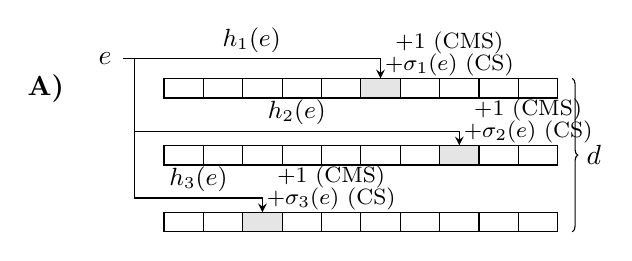
\begin{tikzpicture}
        \def\arraycount{3}
        \def\arrayw{5}
        \def\arrayh{0.25}
        \def\arraylen{10}
        \def\arraysep{0.6}
        \def\counterw{0.5}

        \foreach \i in {1, ..., \arraycount} {
            \draw[black] (0,-\i*\arrayh+1.5*\arrayh-\i*\arraysep+\arraysep) rectangle (\arrayw,-\i*\arrayh+0.5*\arrayh-\i*\arraysep+\arraysep);
            \foreach \j in {2, ..., \arraylen} {
                \draw (\j*\counterw-\counterw,-\i*\arrayh+1.5*\arrayh-\i*\arraysep+\arraysep) -- (\j*\counterw-\counterw,-\i*\arrayh+0.5*\arrayh-\i*\arraysep+\arraysep);
            }
        }
        \draw[decorate,decoration={brace,raise=1pt,amplitude=2pt}] (\arrayw+0.25*\arraysep,0.5*\arrayh) -- (\arrayw+0.25*\arraysep,0.5*\arrayh-\arraycount*\arrayh-\arraycount*\arraysep+\arraysep) 
            node[pos=0.5,right=5pt,inner sep=1pt] (row_count_label) {$d$};
        \node[inner sep=4pt] (element) at (-1.5*\counterw,1.5*\arrayh) {$e$};
        \draw[-stealth] (element.east) -| (5.5*\counterw,0.5*\arrayh) node[pos=0.25,above=2pt,align=center,inner sep=0pt] {\small $h_1(e)$};
        \draw (element.east) -| (-0.75*\counterw,-1.5*\arrayh-1.7*\arraysep);
        \draw[-stealth] (-0.75*\counterw,-0.5*\arrayh-0.7*\arraysep) -| (7.5*\counterw,-0.5*\arrayh-1.0*\arraysep) node[pos=0.25,above=2pt,align=center,inner sep=0pt] {\small $h_2(e)$};
        \draw[-stealth] (-0.75*\counterw,-1.5*\arrayh-1.7*\arraysep) -| (2.5*\counterw,-1.5*\arrayh-2.0*\arraysep) node[pos=0.25,above=2pt,align=center,inner sep=0pt] {\small $h_3(e)$};

        \draw[fill=gray!20] (5.0*\counterw,0.5*\arrayh) rectangle (6.0*\counterw,-0.5*\arrayh);
        \draw[fill=gray!20] (7.0*\counterw,-0.5*\arrayh-1.0*\arraysep) rectangle (8.0*\counterw,-1.5*\arrayh-1.0*\arraysep);
        \draw[fill=gray!20] (2.0*\counterw,-1.5*\arrayh-2.0*\arraysep) rectangle (3.0*\counterw,-2.5*\arrayh-2.0*\arraysep);

        \node[inner sep=0pt,anchor=south west,align=center] at (5.6*\counterw,0.6*\arrayh) {\footnotesize $+1$ (CMS) \\[-4pt] \footnotesize $+\sigma_1(e)$ (CS)};
        \node[inner sep=0pt,anchor=south west,align=center] at (7.6*\counterw,-0.4*\arrayh-1.0*\arraysep) {\footnotesize $+1$ (CMS) \\[-4pt] \footnotesize $+\sigma_2(e)$ (CS)};
        \node[inner sep=0pt,anchor=south west,align=center] at (2.6*\counterw,-1.4*\arrayh-2.0*\arraysep) {\footnotesize $+1$ (CMS) \\[-4pt] \footnotesize $+\sigma_3(e)$ (CS)};

        \node[inner sep=0pt] at (-3.0*\counterw,0) {\textbf{A)}};
    \end{tikzpicture}
    \vspace{8pt}

    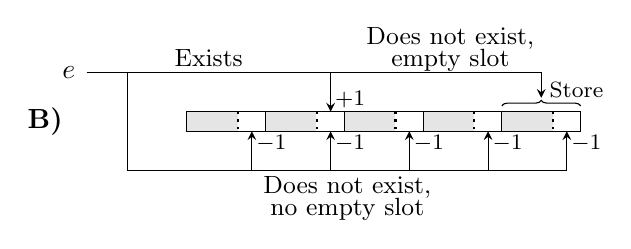
\begin{tikzpicture}
        \def\arrayw{5}
        \def\arrayh{0.25}
        \def\arraylen{5}
        \def\cellw{1.0}
        \def\elemw{0.65}
        \def\counterw{0.35}
        \def\annotationoffset{0.05}
        \def\bottomymul{2.5}

        \foreach \j in {1, ..., \arraylen} {
            %\draw[white,pattern=north east lines] (\j*\cellw-\counterw,0.5*\arrayh) rectangle (\j*\cellw-\cellw,-0.5*\arrayh);
            \draw[white,fill=gray!20] (\j*\cellw-\counterw,0.5*\arrayh) rectangle (\j*\cellw-\cellw,-0.5*\arrayh);
            \draw[dotted,thick] (\j*\cellw-\counterw,0.5*\arrayh) -- (\j*\cellw-\counterw,-0.5*\arrayh);
        }
        \foreach \j in {2, ..., \arraylen} {
            \draw (\j*\cellw-\cellw,0.5*\arrayh) -- (\j*\cellw-\cellw,-0.5*\arrayh);
        }
        \draw[black] (0,0.5*\arrayh) rectangle (\arrayw,-0.5*\arrayh);

        \node[inner sep=4pt] (element) at (-1.5*\cellw,2.5*\arrayh) {$e$};

        \draw[-stealth] (element.east) -| (1.0*\cellw+\elemw+0.5*\counterw,0.5*\arrayh) node[pos=0.25,above=2pt,align=center,inner sep=0pt] {\small Exists};
        \node[inner sep=0pt,anchor=south west] at (1.0*\cellw+\elemw+0.5*\counterw+\annotationoffset,0.65*\arrayh) {\footnotesize $+1$};

        \draw[-stealth] (element.east) -| (\arraylen*\cellw-0.5*\cellw,1.2*\arrayh) node[pos=0.4,above=0pt,align=center,inner sep=0pt] {\small Does not exist, \\[-4pt] \small empty slot};
        \node[inner sep=0pt,anchor=south west] at (\arraylen*\cellw-0.5*\cellw+2*\annotationoffset,1.2*\arrayh) {\footnotesize Store};

        \draw[decorate,decoration={brace,raise=1pt,amplitude=2pt}] (\arraylen*\cellw-\cellw,0.65*\arrayh) -- (\arraylen*\cellw,0.65*\arrayh);
        \draw (element.east) -| (-0.75*\cellw,-\bottomymul*\arrayh);
        \draw (-0.75*\cellw,-\bottomymul*\arrayh) -- (\arraylen*\cellw-0.5*\counterw,-\bottomymul*\arrayh) node[pos=0.5,below=2pt,align=center,inner sep=0pt] {\small Does not exist, \\[-4pt] \small no empty slot};
        \foreach \j in {1, ..., \arraylen} {
            \draw[-stealth] (\j*\cellw-0.5*\counterw,-\bottomymul*\arrayh) -- (\j*\cellw-0.5*\counterw,-0.5*\arrayh);
            \node[inner sep=0pt,anchor=north west] at (\j*\cellw-0.5*\counterw+\annotationoffset,-0.65*\arrayh) {\footnotesize $-1$};
        }

        \node[inner sep=0pt] at (-1.8*\cellw,0) {\textbf{B)}};
    \end{tikzpicture}
    \caption{welp}
    \vspace{-3mm}
    \label{fig:sketches_overview}
\end{figure}

\textbf{Count-Min Sketch (CMS).}
CMS arranges~$d$ independent arrays of~$w$ counters in a~$d \times w$ matrix.
It employs~$d$ hash functions~$h_1,\dots,h_d$, one per array in the matrix. For
an incoming insertion~$e$, CMS iterates through each of the~$d$ arrays,
hashes~$e$ using the corresponding hash function~$h_i$ to map it to a counter,
and increments it. \Cref{fig:sketches_overview}-A) showcases this process. A
deletion for item~$e$ is handled analogously by iterating through the arrays
and decrementing the counters it maps to.

Due to hash collisions, multiple elements can hash to the same counters. As
such, each counter~$e$ hashes to provides an overestimation of its number of
occurrences~$f(e)$. CMS controls this overestimation error by reporting the
minimum counter value across all arrays\footnote{To ensure that this reduces
the estimation error, CMS uses pairwise-independent hash functions, providing a
bound on the probability of overestimation.}.

Letting~$\epsilon=\frac{e}{w}$ and $\delta=e^{-d}$, CMS ensures that, for any
item~$e$, its estimate~$\hat{f}(e)$ is off from~$f(e)$ by at most~$\epsilon N$
with a probability of at least~$1-\delta$, i.e., $\Pr\left( |\hat{f}(e)-f(e)|
\leq \epsilon N \right) \geq 1-\delta$. In other words, CMS errs beyond this
threshold with an error probability of at most~$\delta$.

\textbf{Count Sketch (CS).}
Even though CMS provides bounded errors, its estimations are biased upwards. In
contrast, CS provides unbiased estimations. It also provides universality: the
ability to estimate any function of the frequencies from a large class. Due to
these qualities, CS has been used in many realted tasks in databases and
networks applications, such as table join size
estimation~\cite{Compass,QueryOptimizationSketches} and DDoS
detection~\cite{UnivMon}.

Similarly to CMS, CS employs~$d$ arrays of counters in a~$d \times w$ matrix
and associates a hash function~$h_i$ to each. Additionally, it associates a
hash function~$\sigma_i$ to each array that maps a given item to an ``update
increment'' from the set~$\{-1,+1\}$\footnote{The~$\sigma_i$ form a 4-wise
independent family of hash functions, yielding a bound on the probability of
large errors.}. CS inserts an incoming item~$e$ by iterating through the
arrays, mapping it to a counter, and adding the increment~$\sigma_i(e)$ to the
counter, as illustrated in~\Cref{fig:sketches_overview}-A). It deletes an
item~$e$ by following a similar procedure and subtracting the
increments~$\sigma_i(e)$ from the counters.

Given an item~$e$, it derives a frequency estimate from each array by fetching
the corresponding counter and multiplying its value by~$\sigma_i(e)$. In doing
so, the expected net effect of other items mapping to the same counter remain
zero, while the expected effect of item~$e$ remains the same as~$f(e)$. Like
CMS, however, hash collisions may degrade the accuracy of this estimate. To
control this, CS repeats this operation for all arrays and returns the median
of the values it collects as the estimate~$\hat{f}(e)$.

As with CMS, letting~$\epsilon=\sqrt{\frac{e}{w}}$ and $\delta=e^{-d}$, CS
ensures that, for any item~$e$, its estimation error is not more than~$\epsilon
\cdot \sum_{e'} f^2(e')$ with a probability of at least~$1-\delta$, i.e.,
$\Pr\left( |\hat{f}(e)-f(e)| \leq \epsilon \cdot \sum_{e'} f^2(e') \right) \geq
1-\delta$. Here, $\sum_{e'} f^2(e')$ corresponds to the~$L_2$-norm of the item
frequencies in the stream, whereas~$N$ in the case of CMS is the~$L_1$-norm of
the item frequencies. The~$L_2$-norm is a smaller quantity than the~$L_1$-norm
when the frequency distribution is less skewed.

\textbf{Misra-Gries (MG).}
The accuracy of CMS and CS degrades as the workload becomes more skewed. In
contrast, MG is able to guarantee much lower errors under extreme skew. Because
of this, MG has seen widespread use as a sub-component in many sketch
designs~\cite{BatchUpdateMisraGries,AugmentedSketch,BitMatcher,BubbleSketch,HeavyGuardian,HeavyKeeper,JigsawSketch,MVSketch,SketchVisor,WavingSketch,MicroscopeSketch,PSketch},
and has been implemented in the popular Apache DataSketches
library~\cite{DataSketches}. Although several variations of MG enjoy more
accurate estimations in practice~\cite{SpaceSaving,UnbiasedSpaceSaving}, we
describe MG for simplicity.

MG maintains an array of item and counter pairs.
\Cref{fig:sketches_overview}-B) shows an example of such an array. Here, each
slot in the array is split into a gray and a white part, storing an item
identifier and its frequency count, respectively. The slots in this array are
initialized as empty slots. MG inserts an incoming item~$e$ by first checking
if it has an entry in the array. If it does, MG increments the corresponding
counter of that entry. If~$e$ does not exist in the array and the array has an
empty slot, MG records~$e$ in it along with a frequency counter of~$1$. If $e$
does not exist in the array and the array is full, MG decrements all the
counters in its array. As a result, several counters may become zero, the slots
of which are emptied to make room for new insertions. Emptying slots in this
way bars MG from supporting deletes without introducing severe overestimation
errors. \Cref{fig:sketches_overview} illustrates how MG handles insertions.

Given a query item~$e$, MG checks if it exists in the array. If it does, the
value of its counter is returned as its frequency estimate~$\hat{f}(e)$. If it
does not exist, MG returns an estimate of zero. Observe how MG only
underestimates the frequency of a counter, as it only increments the counter
of an item if it exists in the array and decrements counters otherwise.

\textbf{Comparison.}

\section{Problem Analysis}\label{sec:problem_analysis}

\section{Sketchbook}\label{sec:sketchbook} 

\subsection{Expanding Rows}\label{sec:expanding_rows}

\subsection{Expanding Counters}\label{sec:diva_dynamic}

\section{Theoretical Analysis}\label{sec:theoretical_analysis}

\section{Evaluation}

\textbf{Platform.}
We run experiments on a Fedora 39 machine with an Intel Xeon w7-2495X processor
(4.8 GHz) with 24 cores and 48 hyper-threads. Our machine has a 1920 KB L1, a
48 MB L2, and a 45 MB L3 cache, along with 64 GBs of main memory. 

\section{Related Work}

\section{Conclusion}

%\begin{acks}
%\end{acks}

%\clearpage

\bibliographystyle{ACM-Reference-Format}
\bibliography{sketchbook}


%\appendix

\end{document}
\endinput
